\documentclass[12pt,a4paper]{article}

% Encodage et polices
\usepackage[utf8]{inputenc}
\usepackage[T1]{fontenc}

% Packages mathématiques et symboles
\usepackage{amsmath,amssymb,amsfonts}

% Gestion de la mise en page
\usepackage{geometry}
\geometry{margin=2.5cm}

% Interligne
\usepackage{setspace}
\onehalfspacing

% Hyperliens et images
\usepackage{hyperref}
\usepackage{graphicx}

\title{Analyse Statistique d'un Corpus Poétique}
\author{José Manuel Rodríguez Caballero}
\date{\today}

\begin{document}
	
	\maketitle
	\tableofcontents
	
	%============================================================
	\section{Description du Jeu de Données}
	%============================================================
	
	Le corpus étudié se compose de poèmes provenant de différents auteurs, 
	dont certains sont reconnus comme suicidaires. Plusieurs étapes de nettoyage 
	ont abouti à un ensemble final de données, organisé selon \textbf{quatre niveaux} :
	
	\begin{enumerate}
		\item \textbf{Cas-Témoin} : identifiés par \texttt{pair\_id} 
		(chaque poète suicidaire est apparié à un poète non suicidaire).
		\item \textbf{Poète} : chaque auteur est décrit par diverses informations biographiques 
		(dates, pays, orientation, etc.) et par un indicateur \texttt{suicidal}.
		\item \textbf{Poème} : chaque recueil de vers possède une période (\texttt{Early}, \texttt{Middle}, 
		\texttt{Later}), un titre, etc.
		\item \textbf{Vers} : unité de base pour la mesure des émotions (colère, joie, tristesse, etc.).
	\end{enumerate}
	
	\subsection{Étapes de constitution}
	\paragraph{\texttt{raw\_data.csv}}  
	Fichier de départ (42 lignes), chaque ligne représentant un poème, 
	avec des métadonnées (dates, pays, lien source, etc.).
	
	\paragraph{\texttt{clean\_data\_1.csv}}  
	Fichier intermédiaire où chaque vers est placé sur une ligne 
	(2931 lignes au total). Les informations du poète sont dupliquées 
	pour chaque vers du même auteur.
	
	\paragraph{\texttt{clean\_data\_2.csv}}  
	Fichier final à granularité identique (1 vers par ligne), 
	où le texte du vers est remplacé par des scores émotionnels 
	(\texttt{anger}, \texttt{joy}, \texttt{sadness}, etc.).
	
	\subsection{Données manquantes}
	\begin{itemize}
		\item Les 10 scores d’émotions ne comportent aucune valeur manquante.
		\item Au niveau Poète, la variable \texttt{heterosexual} contient 2 valeurs manquantes (\texttt{NA}).
		\item Les autres champs (dates, pays, etc.) sont complets. 
	\end{itemize}
	Le nombre de valeurs manquantes étant très faible, on considère que cela n’entrave pas l’analyse.
	
	%============================================================
	\section{Présentation des Variables}
	%============================================================
	
	\subsection{Niveau Cas-Témoin}
	\begin{itemize}
		\item \texttt{pair\_id} : identifiant de la paire (poète suicidaire vs. poète témoin).
	\end{itemize}
	
	\subsection{Niveau Poète}
	\begin{itemize}
		\item \texttt{poet} : nom de l’auteur (14 distincts).
		\item \texttt{suicidal} : \texttt{TRUE} ou \texttt{FALSE} (7 de chaque).
		\item \texttt{sex} : \texttt{Male} / \texttt{Female}.
		\item \texttt{heterosexual} : \texttt{TRUE} / \texttt{FALSE} / \texttt{NA}.
		\item \texttt{date\_of\_birth}, \texttt{date\_of\_death} : dates.
		\item \texttt{country\_of\_birth} : pays.
	\end{itemize}
	
	\subsection{Niveau Poème}
	\begin{itemize}
		\item \texttt{period} : \texttt{Early}, \texttt{Middle} ou \texttt{Later}.
		\item \texttt{poem\_title} : titre du poème.
	\end{itemize}
	
	\subsection{Niveau Vers}
	\begin{itemize}
		\item \texttt{anger}, \texttt{anticipation}, \texttt{disgust}, \texttt{fear}, 
		\texttt{joy}, \texttt{sadness}, \texttt{surprise}, \texttt{trust}, 
		\texttt{negative}, \texttt{positive} : scores d’émotions.
		\item Chacune de ces variables est un compteur ou une pondération de mots 
		associés à l’émotion concernée.
		\item Nombre d'observations : 2931
	\end{itemize}
	

	
	%============================================================
	\section{Analyse avec Réduction de la Dimension}
	%============================================================
	
	\subsection{Principe}
	L’analyse statistique se concentre sur les \textbf{moyennes d’émotions par poète}. 
	Pour chaque auteur, on agrège (par la moyenne) les 10 scores d’émotions 
	sur l’ensemble de ses vers, formant ainsi un vecteur dans $\mathbb{R}^{10}$. 
	On obtient donc une matrice $M$ de dimension $14 \times 10$ (14 poètes, 10 émotions).
	
	\subsection{Analyse en Composantes Principales (ACP)}
	\paragraph{Standardisation}
	Avant l’ACP, on ``centre-réduit'' les 10 colonnes d’émotion, 
	afin de les ramener à une moyenne nulle et un écart-type unitaire.
	
	\paragraph{Décomposition}
	Soient $\lambda_1 \ge \lambda_2 \ge \dots \ge \lambda_{10}$ 
	les valeurs propres de la matrice de covariance de $M$. Les composantes principales 
	(PC1, PC2, etc.) sont les vecteurs propres associés, ordonnés par importance décroissante.
	
	\paragraph{Résultats}
	\begin{itemize}
		\item \textbf{PC1 et PC2} : Les deux premières composantes expliquent environ 77,7\,\% 
		de la variance (50,4\,\% pour PC1, 27,5\,\% pour PC2).
		\item \textbf{Position des poètes} : En projetant chaque poète dans le plan (PC1, PC2), 
		on peut observer d’éventuelles tendances de regroupement selon \texttt{suicidal}.
		Aucune séparation claire n’est obligatoirement visible, 
		mais des indices de différences émotionnelles peuvent se dégager.
	\end{itemize}
	
	\begin{figure}[htbp]
		\centering
		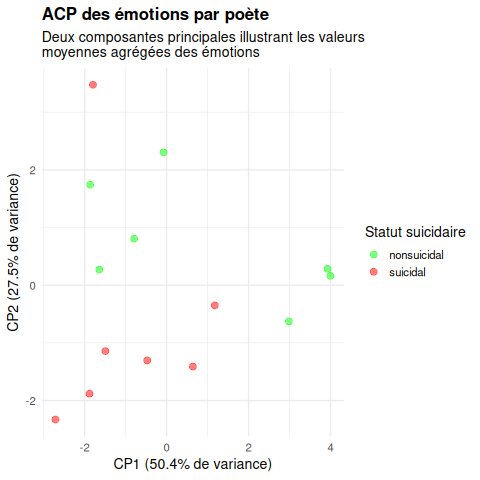
\includegraphics[width=0.65\textwidth]{pca_plot.png}
		\caption{Représentation des poètes dans le plan défini par les deux premières composantes principales (PC1 et PC2). Les couleurs indiquent par exemple le statut suicidaire.}
		\label{fig:pca_plot}
	\end{figure}
	
	
	%============================================================
\end{document}
